\chapter{Hidden Markov Models (HMMs)}
\label{chap:chap10}

\begin{quote}
    Provide a literature review of Hidden Markov Models, in general, and their applications in music information retrieval. [3–5 pages]
\end{quote}
\clearpage

% \section{Markov processes}

% A Markov process is a \emph{memoryless}, stochastic process. Given its current state, it does not require to know the previous state in order to estimate the possible next states of the process. Another way of thinking of it, is that in a Markov process, the future does not depend on the past, only on the present.

% The scientific foundations of such processes were first described by A. A. Markov in the beginning of the XX century \cite{markov_rasprostranenie_1906} and, since they were first coined as \emph{Markov chains} in 1926 \cite{bernstein_sur_1927}, bear Markov's name up until our days.

% \section{Hidden Markov Model}

% Although the theory of Markov chains has been known for that long, it started seeing practical applications around the 1970s and 1980s.

% In the development of Hidden Markov Models, the work by Viterbi \cite{viterbi_error_1967} and the Viterbi algorithm \cite{forney_viterbi_1973} are very important.

% An introduction to Hidden Markov Models \cite{rabiner_introduction_1986} and a famous tutorial on Hidden Markov Models \cite{rabiner_tutorial_1989} can be found.

% During the years 1906-7, A. A. Markov published about a probabilistic framework that he called \emph{chains}.
% By 1922, they started to be known as \emph{Markov chains}.
% During the 1970s, Markov chains saw a big growth in real applications due to the use of computers.
% Several concepts derivated from this theory, for example, the Markov property and a Markov process.
% One of these variants of Markov chains is the Hidden Markov Model (HMM).

The term Hidden Markov Model (HMM) refers to a type of learning algorithm inspired by the work of Andrey Andreyevich Markov (1856--1922) in probabilistic frameworks, originally referred to them as \emph{chains} by Markov but that we know today as \emph{Markov chains}.


\section{A. A. Markov and the Markov chains}
Andrey Andreyevich Markov was a Russian mathematician from the XIX century.\footnote{Not to confuse with Andrei Andreevich Markov (1909--1897), his son, who was also a mathematician.} He was born in the town of Ryazan but moved with his family to Saint Petersburg as a child, where he spent most of his life.

At the age of 18, he started studying at Saint Petersburg University and became a disciple of the famous mathematician Pafnuty Chebyshev. Eventually, in 1886 and being 30 years old, Markov himself became a professor at Saint Petersburg University, continuing a tradition of exceptional academics in the field of probability that included Bernoulli, Bunyakovsky, Chebyshev, and others.

Aside his academic contributions, Markov was an active political activist in a politically-unstable Russia. He refused tsarist awards as a protest, rejected the appointment of royal diplomats as academics when he considered they did not meet the required achievements, and in 1912, he asked to be excommunicated from the Russian Orthodox Church through a letter sent to the holy synod.\footnote{The holy synod replied to his petition and did excommunicate him.}

In terms of his academic career, Markov contributed to mathematics with over 120 papers, primarily in probability, statistics, number theory, continuous fraction theory, and differential equations.

He is particularly remembered for what is known today as \emph{Markov chains}.

\section{Markov chains}

A Markov chain is a model that describes a stochastic process through a sequence of states and transition probabilities between those states. In order to be considered a Markov chain, the probabilities of one state transitioning to another state should depend exclusively in the current state (i.e., the system is \emph{memoryless}, as it does not require information about the past to predict the future, only information about the present).

Although the idea behind Markov chains can already be traced in the work of others like Laplace, Bernoulli, Ehrenfest, Bunyakovsky, and Bachelier \cite{basharin_life_2004}, it consolidated with the paper published in 1906 by Markov \cite{markov_rasprostranenie_1906}.\footnote{The paper was submitted in 1906, however, by the time it was published, Markov managed to write and include a few additional sections.}

It has been argued that the dedication and effort that Markov put into this work was an incidental process, as Markov was trying to prove that Nekrasov (a long-time academic adversary) was wrong when, in 1928, he claimed that ``independence is a necessary condition of the law of big numbers''. Markov studied the law of large numbers in specific sequences of random variables that lead to the creation of a new framework. In his original paper, Markov referred to the probabilistic framework as \emph{chains}, and these chains became a new field of research.

In 1926, four years after the death of Markov, the term \emph{Markov chains} was first used in a paper by Bernstein \cite{bernstein_sur_1927}, and the convention of naming the chains after Markov consolidated over the years, giving raise to related concepts like \emph{Markov process}, the \emph{Markov property}, \emph{Markovian}, and \emph{Hidden Markov Models}, all of which borrow A. A. Markov's name and acknowledge his contribution to the field of \emph{Markov chains}.

\section{Hidden Markov Models}

Hidden Markov Models (HMMs) derivate from the basic idea of a Markov chain, adding the notion of \emph{hidden states}, which allow the study of processes that change over time (e.g., weather, speech, and music). An HMM is able to model such time-varying processes by setting (or training) 5 different parameters. For example, Figure \ref{fig:Q1_1} shows an HMM used for generating melodies that modulate through different musical keys. The 5 parameters of the model are described next.

\begin{figure}[h]
    \centering
    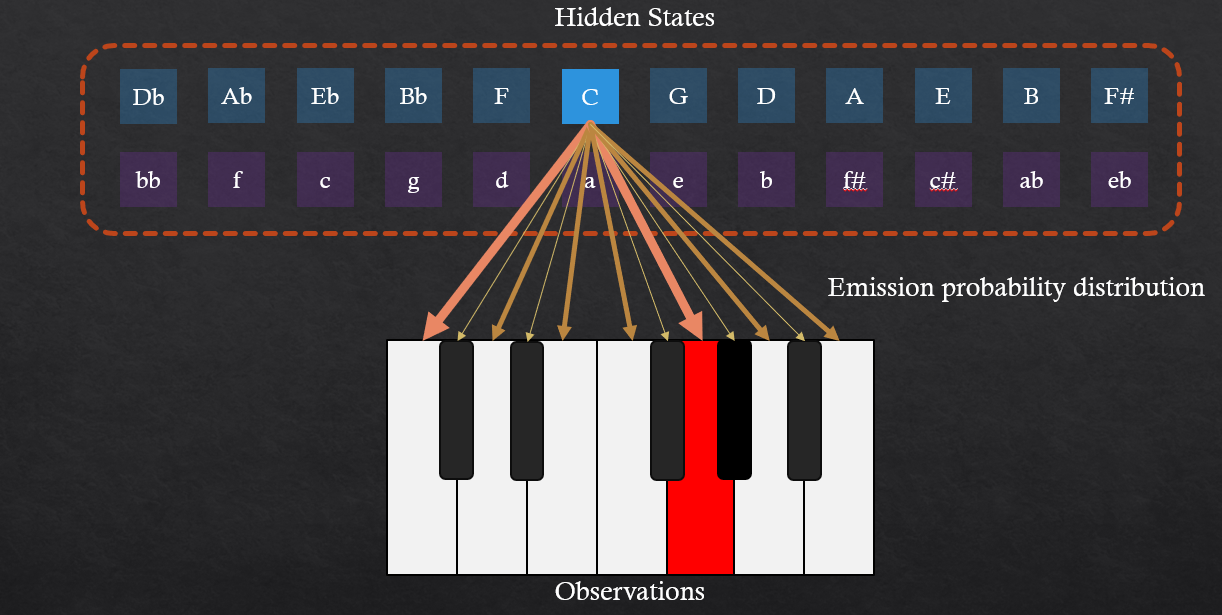
\includegraphics[width=0.8\textwidth]{figures/Q1_1.png}
    \caption{A Hidden Markov Model for generating melodies that modulate through different musical keys. The hidden states consist of the 24 major and minor keys, the observations consist of the notes within the chromatic scale, and the probability distributions are inferred from music theory knowledge.}
    \label{fig:Q1_1}
\end{figure}

%%%%%


 
 Hidden states: these states represent a \emph{steady} behaviour of the system. In the example shown in Figure \ref{fig:Q1_1}, the steady behaviours are different musical keys. Each of the musical keys is expected to produce several notes before they change (modulate) to another key.
 
 Observations: the observations are the outputs emitted by the steady behaviour (hidden state) of the system. In the example shown in Figure \ref{fig:Q1_1}, the observations are the notes, which are produced by a musical key.
 
Initial state probability distribution: this distribution determines how likely is each hidden state when the system first starts. In the example shown in Figure \ref{fig:Q1_1}, the probability of starting in any musical key is the same (i.e., a uniform distribution).

Emission probability distribution: this distribution determines how likely is each of the hidden states to \emph{emit} each of the observations. In the example shown in Figure \ref{fig:Q1_1}, the emission probability represents the probability of a musical key playing a specific note, and it is taken from a perceptual study of tonality \cite{krumhansl_tracing_1982}.

Transition probability distribution: this distribution determines how likely is each of the hidden states to transition to any other hidden state. In the example shown in Figure \ref{fig:Q1_1}, this distribution represents the probability of one musical key \emph{modulating} to another musical key. This distribution is obtained from music-theoretical assumptions \cite{weber_theory_2018}.

%%%%%

An HMM describes a time-varying process through a series of observations that are emitted by a hidden state at each time step. Each hidden state is required to transition to another hidden state after its emission, therefore, a time step concludes once an observation has been emitted by the current hidden state and the current hidden state transitions into a different (or the same) hidden state for the next time step. This process continues for an arbitrary number of time steps.



% The mechanism used to determine the probabilities of a hidden state emitting any observation is called the \emph{emission probability distribution}. Similarly, the mechanism used to determine the probabilities of a hidden state transitioning to any other hidden state (including itself) is called the \emph{transition probability distribution}.

Theoretically, when there is access to real sequences of observations, the emission and transition probability distributions can be ``learned'' automatically from training data, using the \emph{Baum-Welch algorithm} \cite{rabiner_tutorial_1989}. In this case, the HMM is automatically trained to adjust its probability distributions parameters and, possibly, generalize the behaviour of its hidden states for an unseen sequence of observations.

This capability of generalization is what drove the popularity of HMMs in different research fields during the 1960s, gaining the interest of many researchers. The use of computers and the availability of training data made HMMs useful in real applications, for example, speech processing \cite{rabiner_introduction_1986}.

Nowadays, there are modern solutions for modelling time-varying processes that are more powerful than HMMs, particularly, Recurrent Neural Networks (RNNs) (see Question \ref{chap:chap9}). Nevertheless, HMMs are still widely used in research for solving multiple problems that involve sequential data.

Additionally to their applications in speech processing, HMMs have become really popular the in the field of Music Information Retrieval.

\section{HMMs in Music Information Retrieval}

% Audio music classification, Batlle and Cano (2000)
% Audio melody spotting, Durey and Clements (2001)
% Audio music indexing, Jin and Jagadish (2002)
% Audio pitch tracking, Orio and Sette (2003)
% Symbolic roman numeral analysis, Raphael and Stoddard (2003)
% Audio chord labelling, Sheh and Ellis (2003)
% Query by humming, Shifrin and Birmingham (2003)
% Audio chord labeling, Bello and Pickens (2005)
% Query by humming, Jang et al. (2005)
% Audio melody spotting, Pikrakis and Theodoridis (2005)
% Audio instrument recognition, Eichner et al. (2006)
% Audio chord labelling, Lee and Slaney (2006)
% Audio key estimation, Noland and Sandler (2006)
% Audio drum transcription, Paulus (2006)
% Audio key estimation, Peeters (2006)
% Optical music recognition, Pugin (2006)
% Audio chord-and-key detection, Catteau et al. (2007)
% Audio chord-and-key detection, Lee and Slaney (2007)
% Audio chord labelling, Papadopoulos and Peeters (2007)
% Audio drum transcription, Paulus 2007 (Paulus 2006 with added temporal features)
% Optical music recognition, Pugin et al. (2007)
% Pitch-spelling, Teodoru and Raphael (2007)
% Audio chord labelling, Khadkevich and Omologo (2009)
% Music structural segmentation, Paulus (2010)
% Audio chord labelling, Ueda et al. (2010)
% Audio chord labelling, Chen et al. (2012)
% Audio music transcription, Benetos and Weyde (2013)
% Piano fingering, Nakamura et al. (2014)
% Audio music transcription, Jancovic et al. (2015)
% Score following, Narakmura et al. (2015)
% Guitar fingering, Hori and Sagayama (2016)
% Audio music transcription, Cazau et al. (2017)
% Symbolic chord labelling, Masada and Bunescu (2017)
% Audio pitch tracking, Nishikimi et al. (2017)
% Confidence measures in music labelling systems, Pauwels et al. (2017)

Since their introduction to the Music Information Retrieval (MIR) community, in 2000, HMMs have been frequently used for solving multiple problems related with MIR.

More specifically, HMMs have been successfully applied to audio music classification \cite{batlle_automatic_2000},
audio ``melody spotting'' \cite{durey_melody_2001, pikrakis_novel_2005},
audio music indexing \cite{jin_indexing_2002},
audio pitch tracking \cite{orio_hmm-based_2003, cazau_improving_2017},
symbolic roman numeral analysis \cite{raphael_functional_2004},
audio chord labelling \cite{sheh_chord_2003, bello_robust_2005, lee_automatic_2006, papadopoulos_large-scale_2007, khadkevich_use_2009,ueda_hmm-based_2010, chen_chord_2012},
query by humming \cite{shifrin_effectiveness_2003, jang_continuous_2005},
audio instrument recognition \cite{eichner_instrument_2006},
audio key estimation \cite{noland_key_2006, peeters_chroma-based_2006},
audio drum transcription \cite{paulus_acoustic_2006, paulus_combining_2007},
optical music recognition \cite{pugin_optical_2006, pugin_map_2007},
audio chord-and-key estimation \cite{catteau_probabilistic_2007, lee_unified_2007},
symbolic pitch-spelling \cite{teodoru_pitch_2007},
audio structural segmentation \cite{paulus_state_2010},
audio music transcription \cite{benetos_explicit_2013,jancovic_automatic_2015, cazau_improving_2017},
symbolic piano fingering \cite{nakamura_merged-output_2014},
score following \cite{nakamura_autoregressive_2015},
guitar fingering \cite{hori_minimax_2016},
symbolic chord labelling \cite{masada_chord_2017},
and computing confidence measures \cite{pauwels_confidence_2017}.

Although their use has decreased significantly in recent years, it is not uncommon for HMMs to provide state-of-the-art performance in certain MIR tasks.


% \cite{viterbi_error_1967}
% \cite{shifrin_effectiveness_2003}

\bibliographystyle{plain}
\bibliography{zoterorefs}